\chapter{Introduction}~\label{ch01_introduction}

We are doing interesting things with biological filters.  I really don't know what to write in the introduction and that worries me.

\begin{figure}
\centering
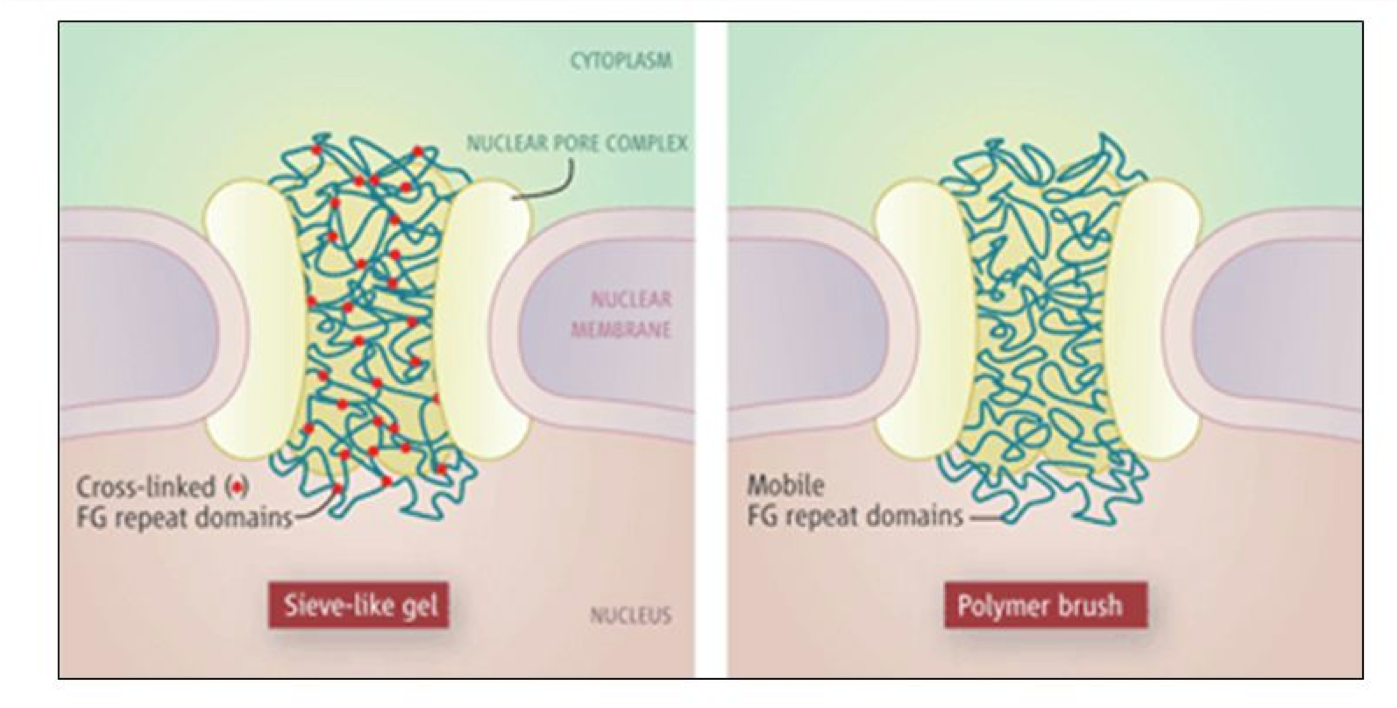
\includegraphics[width=0.7\linewidth]{figs/ch01/elbaum}
\caption{Dependence of selectivity on variation of individual
  parameters: (a) on-rate constant, (b) total FG Nup concentration, (c) inverse of the free diffusion coefficient, and (d) pore
  length, with varying dissociation constant. All values calculated using the linear solution to the binding-diffusion equations.  Bound diffusion coefficient $D_B = 0.1D_F$. Other parameters fixed at values from the NPC parameters section.}
\label{fig:parameter-variations}
\end{figure}




%%%%%%%%%%%%%%%% IDPS %%%%%%%%%%%%%%%%%%

\section{Intrinsically disordered proteins are essential to cellular function}
For decades, it was conventional wisdom among biologists that a protein's folded shape determined its function.  Most enzymes and other proteins that were studied had a stable folded configuration, the lowest point on a well-defined folding energy landscape.  A protein's conformation provided specific docking points through which it could interact with ligands or other proteins in a ``lock-and-key'' model.

However, a few decades ago, it began to become clear that not all proteins have a well-defined ternary or even secondary structure, but rather exist as extended polymer chains.  These intrinsically disordered proteins (IDPs) were initially dismissed as nonfunctional, but evidence began to accumulate that they were in fact essential for cellular function, overturning the structure-function paradigm \cite{uversky13}.  Their roles and importance are still being understood, as are the unusual mechanisms by which they accomplish their functions without a well-defined structure.

Today, it is estimated that 30\% of eukaryotic proteins are disordered or contain significant disordered regions \cite{uversky13}.  While there is significant sequence heterogeneity among IDPs, they tend to contain a large proportion of hydrophilic residues, and often have long stretches of low-complexity regions where only a few amino acids are represented.  They also often have high net charge.

Some IDPs fold (or partially fold) upon binding with an ordered partner, while others form ``fuzzy'' complex that remains disordered.  Their advantages over folded proteins may include their plasticity, which enables them to bind many different binding partners.  Multivalency, either as one-to-many or many-to-one binding, may also play a role.  They may act as hubs that bring together larger complexes.  Similarly, IDPs are often known for having high specificity at relatively weak binding strengths \cite{uversky13}.

While the normal functioning of IDPs is very important to the cell, IDPs are also prone to aggregation and are at the root of pathologies such as Alzheimer's disease, Parkinsons, and prion diseases.  Often, normally-disordered proteins aggregate into amyloid fibrils, a stable structure based on parallel beta-sheets.

IDPs are commonly involved in cell signaling and regulation \cite{uversky13}.  Their disordered nature makes them useful as hubs that bring together many other proteins, and as scaffolds that many proteins can bind to at once.  IDPs appear to be prevalent in transcriptional regulation, and they are playing increasingly apparent roles in liquid-liquid phase separation within cells.  One of the most fascinating examples of IDP function is in the nuclear pore complex (NPC), a unique selective barrier that regulates all transport between the nucleus and the cytoplasm.  The link between disorder and selectivity is not well understood in this case.

%%%%%%%%%%%%%%%%%%% NUCLEAR PORE STRUCTURE %%%%%%%%%%

\section{Major components of nucleocytoplasmic transport}
The nuclear pore complex (NPC) resides in the nuclear envelope of eukaryotes and regulates all macromolecular traffic between the nucleus and cytoplasm.  The NPC is one of the largest protein complexes in the cell, at about 60 MDa in yeast and 120 MDa in humans \cite{beck17}.  As the regulator of nucleocytoplasmic transport, the NPC must rapidly and specifically pass a wide array of macromolecules: transcription factors into the nucleus, and RNA into the cytoplasm.  Moreover, it must be robust to problems and able to accomodate mechanical strain as the nuclear envelope changes shape, and to passage large cargo.

A typical yeast cell has xx nuclear pores, each with a dimension of xx.  Human cells have about xx pores with xx dimensions.

There are about 30 different types of Nups, all present in multiple copy numbers.

These functions are accomplished through a structure with two main parts, both made of proteins known as nucloporins, or Nups: the scaffold Nups, which form a ringlike complex, and the FG Nups, which are disordered and fill the central channel created by the scaffold Nups.  Aside from the NPC itself, transport factors (TFs) are a class of proteins essential for selective transport.  The energetic cost of selectivity is captured in the Ran GTP/GDP cycle.

\subsection{Scaffold nucleoporins are ordered and form ringlike complexes.}
The nuclear pore itself is formed of scaffold Nups, which are ordered proteins that form ringlike complexes with eightfold symmetry \cite{beck17}.  There is an inner ring and two outer rings, the nuclear and cytoplasmic rings.  The outer rings are slightly larger.  The nuclear ring is on the side of the nucleus and includes the nuclear basket.  The cytoplasmic ring includes the cytoplasmic filaments, which are (probably?) disordered proteins extending out into the cytoplasm.

The eightfold symmetry of the pore arises from its modular nature.  Scaffold Nups form various stable subcomplexes, of which one of the most important is the Y-complex.  The Y-complex forms the inner ring; there are 32 copies of the complex per pore \cite{beck17}.  The rings themselves are relatively flexible, as they need to be in order to accomodate deformations of the nuclear envelope.  This flexibility is achieved in part by through short linear motifs (SLMs) which connect the subcomplexes to each other.

Recent cryo-EM studies have achieved unprecedented resolution of the scaffold Nups \cite{rout study, other EM study}.

% Scaffold Nups have very low turnover rates. \cite{knockenhauer16}
% 2000-3000 copies of NPC in an average human cell. \cite{knockenhauer16}
%''The mass flow through NPCs in proliferating HeLa cells is estimated to be 10–20 MDa·NPC−1·s−1 `` verbatim from \cite{tu11}
% Largest cargos are 40 nm also has a citation in Tu SM review article 2011

\subsection{FG nucleoporins are disordered and fill the central channel of the pore.}
The central channel of the pore is filled with disordered FG nucleoporins (FG Nups).  FG Nups typically consist of an ordered domain that anchors them to the wall of the channel, and an entirely disordered domain that extends into the channel.  As with all Nups, FG Nups have eightfold symmetry in the pore, and some of them are present in much higher copy number.

The disordered portion of every FG Nup contains phenylalanine- glycine (FG) motifs which 
bind to the hydrophobic binding pockets of transport factors.  While there are multiple binding motifs, all are short sequences which incorporate an FG repeat; for instance, FSFG, GLFG, and others. \cite{the rout paper I took that figure from}.  Each FG Nup contains x-x FG repeats, leading to an extremely high density of FG repeats within the pore.

Since the FG Nups are disordered, most conventional visualization techniques do not work.  When imaged over time or when several pores are imaged, the averaged results do not show the disordered portion of the FG Nups.  Cryo-EM and x-ray crystallography don't work.  Techniques such as NMR and very fast AFM can help gain insight into their conformationa ensembles \cite{Loren's papers, the AFM paper}.  Early research suggested that the FG Nups formed a central plug or "transporter", but more recent work suggests that there is no central structure, just disordered proteins (the AFM study from Lim or Lemke group). There is some evidence from simulations that the density of the FG Nups, as well as their charge density and hydrophobic properties, are not uniform along either the radial or axial directions \cite{some energy landscape things, some simulations}.  This may contribute to selective transport, although the pore still functioned with all of the asymmetric FG Nups removed.  Indeed, the NPC is remarkably robust to FG Nup deletion.  Over half of the mass of FG Nups can be removed without eliminating the selectivity barrier \cite{beck17}.

\subsection{Energy for selective transport is provided by the Ran cycle.}
Selective transport requires an energy source, which in the case of the NPC is provided by the Ran cycle.  When a TF-cargo complex passes from the cytoplasm into the nucleus (nuclear import), it encounters a RanGTP on the nuclear side which binds to the TF and displaces the cargo.  Then the TF-RanGTP complex can collect a cargo destined for nuclear export, and this ternary complex can diffuse back through the NPC to the cytoplasm.  The protein RanGAP then hydrolyzes the RanGTP to RanGDP, disrupting the complex into its three original pieces.  Ultimately, the energy source for selective nuclear transport comes from the RanGTP-RanGDP gradient from the cytoplasm to the nucleus, a gradient which is maintained partially by NTF2, which carries RanGDP through the pore \cite{stanley17}.

From the perspective of transport, this means that the process of passing through the pore is itself passive and does not consume energy.  The selectivity arises from concentration gradients maintained by the Ran cycle.

\subsection{Transport factors}

Transport factors (TFs) are ordered proteins that carry cargo through the NPC.  While there are various types, they share several features in common, most notably the fact that all known transport factors have more than one hydrophobic binding pocket which binds to FG repeats.  In fact, many TFs have several binding pockets.  Likewise, the binding affinity between TFs and FG Nups remains unknown for most TFs.  Estimates of dissociation constant $K_D$ vary from nanomolar to millimolar, depending on the environment (cellular, buffer, etc.) in which the measurement is made \cite{things}. There are many types of TF, of which some of the most important are the importins and exportins (karyopherins), NTF2, (and mRNA exporters? CRM? mex67?).

The karyopherins (Kaps) are the most-studied family of TFs.  They are also known (in human cells?) as importins and exportins, or collectively as the importin $\beta$ superfamily \cite{tu11}.  The twenty or so different Kaps are responsible for most nucleocytoplasmic transport \cite{kapinos17}.  Kaps typically consist of multiple HEAT repeats, a helical motif which conveys structural flexibility \cite{yoshimura16}.  Most Kaps bind their cargo directly via a nuclear localization signal (NLS, for nuclear import) or nuclear export signal (NES, for nuclear export).  NLS and NES are 5-7 amino acid tags found on cargo \cite{}.  However, Kap95? (importin $\beta$) uses the adaptor protein Kap60? (importin $\alpha$) to bind its cargo. In general, Kaps are on the order of 100 kDa in size, well above the passive permeability limit \cite{}. Kaps may contribute to the selectivity barrier.

Unlike the karyopherins, nuclear transport factor 2 (NTF2) does not transport a wide variety of cargo across the NPC.  Instead, NFT2 is focused on maintaining the Ran gradient needed for transport.  It transports RanGDP across the pore - why does this help maintain a gradient?  If it transports in both directions, wouldn't it help wash out the gradient?  NTF2 is a homodimer whose components are 14 kDa and have one FG binding site.  Although its small size of 28 kDa is near the 30 kDa cutoff for passive transit through the pore, its flux through the pore is still 30-150 that of similarly-sized proteins that do not bind to FG Nups.

There are other TFs such as Mex67 and CRM, but I don't really know what they do.  Is RNA exported using Kaps or are there other TFs for that?

%%%%%%%% EXPERIMENTAL OBSERVATIONS %%%%%%%%%%%%%%%
%\section{Observed features of nucleocytoplasmic transport}
%\subsection{Flux through the NPC is very high.}
%\subsection{TFs show millisecond dwell times.}
%\subsection{TF-FG Nup binding kinetics are ultrafast.}
%\subsection{FG Nups may take a variety of conformations.}
%    \subsubsection{Grafted layer heights change when TFs are added.}
%    \subsubsection{Inter-Nup cohesion varies between FG Nups.}
%\subsection{TF concentration and crowding may affect selectivity.}
%\subsection{The NPC is also a passive permeability barrier.}
%\subsection{A detailed, mechanistic picture of selective transport is still unclear.}


\section{Observed features of nucleocytoplasmic transport} 
The nuclear pore has been the subject of investigation since the 1950s \cite{hapensomething16 or another review article with timeline}.  During that time, many different experimental techniques have been used, from in vivo studies to single molecule fluoresecence to SPR to NMR.  Likewise, simulations have attempted to explain the selectivity properties of the NPC using a broad array of techniques, such as more or less coarse-grained molecular dynamics simulations.  These studies together shed light on the mechanisms of selective transport, but are also all hindered by the small size and rapid timescale of transport.  Many of the studies produce results that seem, at least at first glance, to contradict those of other studies.  A comprehensive picture of the facts of nuclear transport has yet to emerge, although there are some universally accepted features.

\subsection{Flux through the NPC is very high.}
The high macromolecular traffic between nucleus and cytoplasm requires high flux through each NPC.  Experiments with permeabilized cells estimate that the total molecular flow through the NPC could be as high as 10-20 MDa per pore per second, corresponding to roughly 1000 transport events per pore per second \cite{ribbeck01}.  Experiments focusing particularly on NTF2 report fluxes between 50 and 250 molecules per pore per second \cite{ribbeck01, siebrasse02, kiskin03}.  Fluxes this high mean a continuously high occupancy of the NPC, estimated at around 100 karyopherins at once \cite{paradise07}.  It is unclear whether the effect of crowding with TFs in the pore has an impact on selectivity.

\subsection{TFs show millisecond dwell times.}
One reason that individual NPCs can accomodate such high flux is the rapidity with which molecules transit the pore.  A wide range of molecules, such as NTF2, Importin $\beta$, and GFP-NLS cargoes, have a dwell time of less than 10 ms in the pore \cite{tu11, yang06, dange08, kubitscheck05}.  Typically, this is determined using single-molecule tracking with superresolution microscopy \cite{tu11}.  There is some evidence that a subpopulation of karyopherins resides in the pore over long timescales, potentially contributing to the selectivity barrier \cite{kapinos17}.

The flux through an NPC is determined not only by the transit time, but also by the success rate of transit attempts.  Single-molecule microscopy suggests that the nuclear import efficiency of Importin $\beta$ ranges from 50\% to 80\%, depending on concentration \cite{yang06}.  Modeling supports these numbers \cite{zilman07}.

\subsection{TF-FG Nup binding kinetics are ultrafast.}
The short dwell time of transport factors and cargo at the pore contributes to a source of confusion in the NPC community: the binding kinetics of TFs and FG Nups.  Measurements of dissociation constant $K_D$ and its components $\kon$ and $\koff$ ($K_D = \koff/\kon$) span several orders of magnitude, depending on the measurement conditions.  Original in vitro measurements, performed in buffer, show low $K_D$ values in the nanomolar range, indicating tight binding between TFs and FG Nups.  However, these values were not compatible with a transit time around 10 ms, as a typical binding event as calculated from the off-rate would last much longer than 10 ms.

More recent measurements are converging on a consensus that TF-FG Nup binding kinetics are in fact much faster than previously estimated.  Diffusion-limited on-rates and $K_D$ values around 1 mM would permit rapid transit through the pore.

\subsection{Passive permeability barrier}
There is a cutoff around 30 kDa where molecules stop being able to passively transit the pore at any appreciable rate.  Work from the Timney lab suggests that the passive permeability barrier is not a sharp cutoff, but broad.
%\subsection{Single-molecule studies}
%Single-molecule studies can elucidate things like the dwell time of a molecule in the pore or the probability that a transport event is successful.  Since transit is quite rapid and, and the size of the pore is below the diffraction limit, SM studies use super-resolution microscopy with video frame rates of 200-1000 frames/s \cite{tu11}.  Even so, a single SM data point typically has higher error than other methods and should be averaged or combined with other data points for a reliable picture \cite{tu11}.  An advantage of SM studies of the NPC is that the region of interest (NPC) is easy to find with conventional light microscopy, relatively immobile, and the ROI is confined to one plane (the plane of the nuclear envelope) \cite{tu11}.

Dwell times for various TFs and TF-cargo complexes has been studied in many cases, giving a typical dwell time of 5-10 ms, with a small minority of complexes spending much longer in the pore \cite{tu11}.

%
%Some of these studies lead to estimations of the transport kinetics, i.e. on and off rates for Nup and transport factor interactions.  Many of these come from SPR studies or stopped-flow anisotropy measurements.  The SPR measurements also lead to estimations of layer height compaction or extension when various TFs are flowed across a grafted monolayer of FG Nups.  These experiments can often result in contradictory data.  There are some good review articles for single-molecule studies, and also some of the techniques I've described here aren't single molecule.
\subsection{Effect of transport factors}
The presence of transport factors may make the selectivity barrier more robust.  SPR measurements as discussed above give estimates of layer compaction or extension, and populations of tight- or weak-binding TFs.  Other studies (?) suggest that crowding with TFs might help reduce non-specific interactions and increase the selectivity of transport.
\subsection{Permeability barrier/flux studies}
People have measured the flux through the pore in vitro and in vivo in various ways.  One group developed OSTR, where they seal an NPC to the pore of a membrane and measure fluorescence flux of TFs through that pore.  The Gorlich group (Ribbeck) have permeabilized cells and injected fluorescent transport factors and watched how long it took them to localize to the nucleus.  These measurements show selectivities of 20-150 (ish) fold flux of TFs as compared to inert proteins.
%\subsection{Nup deletion, etc.}
%Some people have deleted subsets of Nups to see which are necessary for transport.  I don't know much about these studies.  None of the asymmetric Nups are necessary.  I think that about half of the mass of Nups can be deleted without significant consquences to transport, showing how robust the NPC is.

%%%%%%%%%%% MODELS OF THE NPC %%%%%%%%%%%%%%%%


\section{Theoretical models of the NPC}
Many theoretical models exist, both qualitative and quantitative.
\subsection{Entropic barrier model}
The entropic barrier model postulates that Nups remain disordered within the pore (should talk about experimental evidence for and against).  In this model, inert proteins are kept out of the pore through an entropic barrier, because their entry into the pore would restrict the possible conformations of the disordered Nups.  TFs can get into the pore, in contrast, because the binding energy offsets the entropic penalty.  This is one of the two main qualitative models of the pore, the other being the hydrogel or selective phase model.  The Rout lab supports this model.  I think most labs other than the Gorlich lab are beginning to support this model, but I'm not sure.
\subsection{Hydrogel model}
The hydrogel model is the other main qualitative NPC model.  The Gorlich group supports this model.  This model postulates that the Nups interact via their FG motifs (discuss evidence in previous section, maybe?) and form a hydrogel.  A dynamic hydrogel.  Inert proteins are kept from passing through because they can't get through the gel mesh, but transport factors disrupt the crosslinks by binding to FGs and "melt" through.
\subsection{“Forest”/intermediate models}
This model proposes that a mix of the entropic barrier model and selective phase model are at play.
\subsection{Effect of crowding}
Some people (Zilman paper, etc) have modeled the effect of crowding on the selectivity barrier.  A lot of overlap with effect of transport factors.
\subsection{Effect of transport factors}
Same as previous section sort of.  Kap-centric models of the NPC (short for karyopherin-centric, for the class of TFs called karyopherins) propose that a permanent population of Kaps lives within the NPC.  This strengthens the selectivity barrier.
\subsection{Energy landscape models}
Most quantitative models of the nuclear pore are energy landscape models.  These are typically computational studies that require a fair amount of detail and assumptions about the pore.  They incorporate effects of charge, hydrophobicity, specific binding interactions, etc.  Generally the result is a picture of the free energy landscape encountered by TFs and by inert proteins as the travel along the axis of the pore.
%%%%%%%%%%%%%%%%%%%%%%%%%%%%%%%%%%%%%%%%%%%%%%%%%%%%%%%%%%%%%%%%%%%
\section{Synthetic NPCs have seen limited success.}
Many different groups have attempted to make synthetic nuclear pore complexes, but they are generally not very successful.
\subsection{Gold nanopores (Rout group)}
One of Loren's colleagues in New York grafted FG Nups onto a gold-coated nanopore and monitored flux through the pore.  She saw low (less than 10-fold) selectivity.  I'm not sure whether other nanopore-based approaches have been tried.
\subsection{Hydrogels (Gorlich)}
The Gorlich group keeps making hydrogels out of Nups and testing the entry of various proteins.  They take Nsp1 or fragments of it or other Nups that spontaneously form hydrogels in buffer, and let them form a gel.  Then they introduce fluorescently-tagged TFs and inert proteins and monitor the progression of the fluorescent front into the gel.  They see very high (100 or more) partition coefficients, indicating that the TFs really bind very strongly to the gel.  They do not see rapid exit from the gel as would be required for rapid transport.
\subsection{Other models (peptide hydrogels, DNA origami, etc)}
There are a grab-bag of other models that I need to learn more about.  Some groups have done similar things to what we want to do, making hydrogels out of non-aggregating Nup peptides and a pentameric crosslinking domain.  There was a group that made an NPC ring out of DNA origami and attached Nups at particular points, though I'm not sure how that can be used to test selectivity because I can't see how to anchor the rings into a membrane.
\section{Conclusions of introduction?}
NPCs are interesting and important.

%Alternate introduction outline:
%\section{Intrinsically disordered proteins are essential to cellular function}
%
%\section{The nuclear pore complex is a remarkable filter}
%
%\section{Major components of nucleocytoplasmic transport}
%\subsection{Scaffold nucleoporins comprise the structure of the pore.}
%\subsection{Disordered FG nucleoporins fill the pore and create the selective barrier.}
%\subsection{Transport factors carry cargo through the NPC.}
%    \subsubsection{Karyopherins}
%    \subsubsection{RNA exporters}
%    \subsubsection{Nuclear transport factor 2 (NTF2)}
%\subsection{The Ran cycle powers selective transport.}
%

%
%\section{Models of nucleocytoplasmic transport}
%
%\section{Synthetic nuclear pores have seen limited success.}
%
%\section{Much still remains unknown about selective transport through the NPC.}

